

\section{Performance measures}
In aiding the quantification of the two proposed test groups, a Fitts' law test will be used. A general Fitts' law incorporates five different performance metrics in the evaluation of movement.\cite{Kamavuako2014,Scheme2013} The five metrics and their description can be found in table \ref{fig:Fitts}    

  \begin{figure}[H]                                         
  	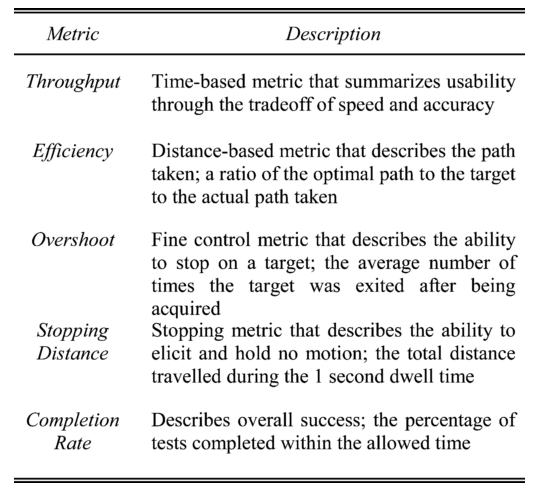
\includegraphics[width=.4\textwidth]{figures/Fitt}  
  	\caption{The table shows the metrics used in a generel Fitts' law test followed by a description of these.\cite{Scheme2013}}
  	\label{fig:Fitts} 
  \end{figure}

Often the throughput ($TP$) is used by its own representing the tradeoff between speed and accuracy. $TP$ uses the relationship of time taken to reach a certain target in seconds ($MT$) and the index of difficulty ($ID$). This forms:\cite{Scheme2013}

\begin{flalign}
TP=1/N\sum_{i=1}^{N} ID_i/MT_i
\label{TP}
\end{flalign}

where $i$ is a specific movement condition and $N$ is the total number of targets. $ID$ relates to the target distance $D$ and width $W$. The $ID$ for each task, from the origin to a specific target of a certain size is calculated using:\cite{Scheme2013}

\begin{flalign}
	ID=log_2(\frac{D}{W}+1)
	\label{ID}
\end{flalign}
 

Put in figure of the GUI used for testing where we represent the number of targets and the distance to them.
Them afterward also calculate the ID for our targets.  

 